\chapter{Phương trình trạng thái, bức xạ và năng lượng chân không}

\lectureoverview{Lịch sử của một vũ trụ đồng nhất phần lớn là lịch sử của hệ số tỉ lệ \(a(t)\). Phương trình Friedmann cung cấp hình học, nhưng phương trình trạng thái của vật chất cho biết mật độ năng lượng thay đổi như thế nào khi không gian giãn nở. Trước hết ta suy ra \(\rho\propto a^{-3(1+w)}\) từ công do một chất lưu thực hiện, rồi thu được \(P=\rho/3\) cho bức xạ bằng cách đếm sự truyền động lượng của photon, và cuối cùng xác định năng lượng chân không qua \(P=-\rho\). Năng lượng chân không dương tạo ra sự giãn nở de Sitter; độ cong và dấu của hằng số vũ trụ học tạo ra các nghiệm nảy bật và tái co sụp có thể được hiểu như những hệ cơ học đơn giản.}

\section{Hệ số tỉ lệ và quy luật vật chất còn thiếu}

Trước hết, ta hãy nhắc lại đích đến của mình. Trong gần đúng đồng nhất và đẳng hướng, lịch sử vũ trụ học chủ yếu được mã hóa trong một hàm, \(a(t)\). Biết hàm đó không trả lời mọi câu hỏi về vũ trụ, nhưng nó quyết định khoảng cách, tốc độ giãn nở và trình tự các thời kỳ ở quy mô lớn. Mục đích của bài giảng này chưa phải là xác lập các thời kỳ ấy bằng quan sát, mà là suy ra, từ vật lý cơ bản, các phương trình trạng thái làm cho các mô hình đó khả dĩ.

Hai mô hình chuẩn đã xuất hiện:
\begin{equation}
a(t)\propto t^{2/3}
\qquad\text{(matter domination)},
\end{equation}
và
\begin{equation}
a(t)\propto t^{1/2}
\qquad\text{(radiation domination)}.
\end{equation}
Không định luật nào đúng chính xác ở mọi thời điểm. Bức xạ cho gần đúng hữu ích ở thời sớm, còn vật chất cho gần đúng ở giai đoạn trung gian muộn hơn; về sau năng lượng chân không lại thay đổi hành vi ở thời muộn. Câu hỏi trước mắt không phải là các quan sát bộc lộ những thời kỳ ấy như thế nào, mà là điều gì phân biệt các vế phải tương ứng của phương trình Friedmann.

\begin{figure}[htbp]
\centering
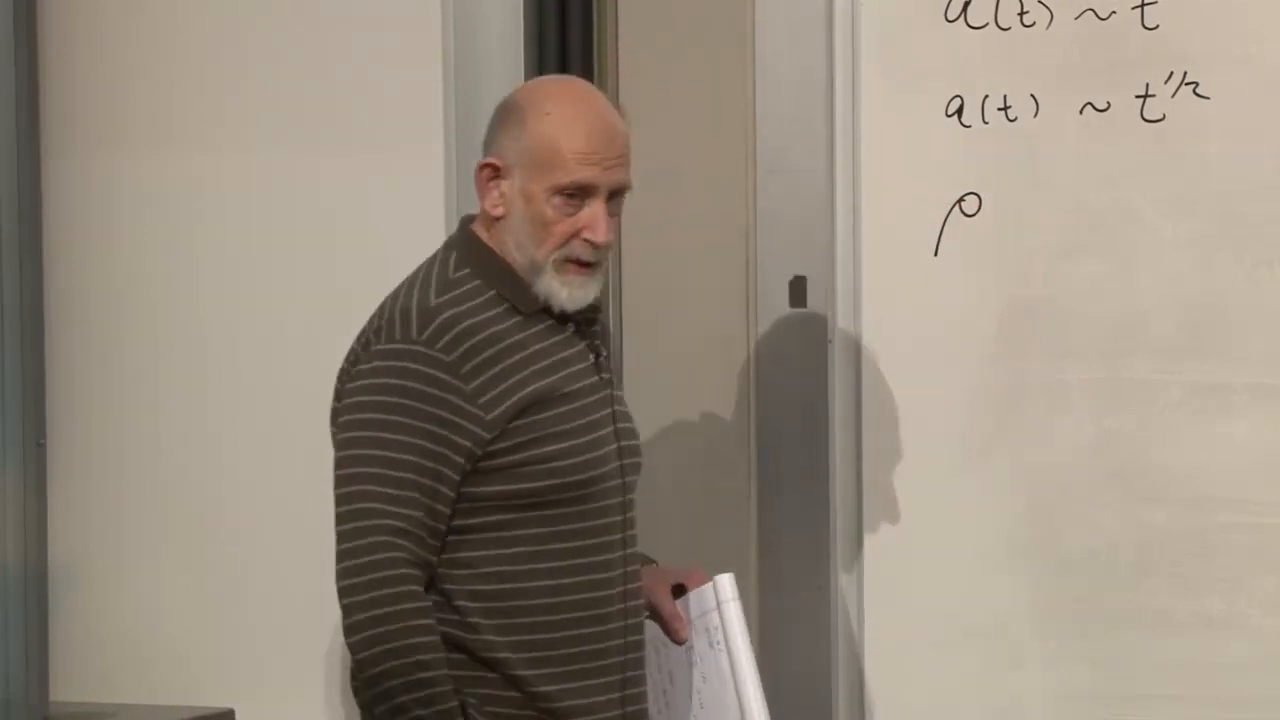
\includegraphics[width=0.72\textwidth]{lecture_05_figure_02.png}
\caption{Các định luật lũy thừa của hệ số tỉ lệ đã được ôn lại và ký hiệu mật độ mới được đưa vào. Đây là trạng thái chuyển tiếp của bảng chứ không phải một phép suy dẫn hoàn chỉnh.}
\label{fig:c05-review-board}
\lectureframe{00:03:18.380}
\end{figure}

Cầu nối còn thiếu là phương trình trạng thái. Nó quyết định mật độ năng lượng ở vế phải của phương trình Friedmann thay đổi như thế nào theo hệ số tỉ lệ. Hai định luật chuẩn là
\begin{equation}
\rho_{\text{matter}}=\frac{\rho_0}{a^3},
\qquad
\rho_{\text{rad}}=\frac{\rho_0}{a^4}.
\label{eq:c05-benchmark-densities}
\end{equation}
Vật chất bị pha loãng theo thể tích, và thể tích tỉ lệ như \(a^3\). Bức xạ giảm thêm một lũy thừa của \(a\). Ta muốn hiểu cả hai quy tắc như những hệ quả của quan hệ giữa áp suất và mật độ năng lượng.

\section{Từ áp suất đến định luật tỉ lệ của mật độ}

Phương trình trạng thái nói chung có thể liên quan đến mật độ, áp suất, nhiệt độ và các biến khác. Đối với các thành phần vũ trụ học được xét ở đây, ta dùng dạng hữu ích với \(w\) không đổi
\begin{equation}
P=w\rho,
\label{eq:c05-eos}
\end{equation}
trong đó \(w\) đặc trưng cho chất lưu. Trên bảng dùng chữ hoa \(W\); ở đây ta dùng chữ thường quy ước \(w\). Dạng tuyến tính này bao quát các trường hợp quan trọng bên dưới, nhưng nó là một giả thiết đơn giản hóa chứ không phải định luật mà mọi chất lưu khả dĩ đều tuân theo.

Đối với vật chất phi tương đối tính, mật độ năng lượng bị chi phối bởi năng lượng nghỉ. Nếu \(n\) là mật độ số và \(m\) là khối lượng hạt, thì về sơ đồ ta có
\begin{equation}
\rho\simeq nmc^2.
\end{equation}
Thừa số \(c^2\) khiến ngay cả một khối lượng nghỉ nhỏ cũng là một kho dự trữ năng lượng khổng lồ; sự hủy hoàn toàn của một hạt bụi sẽ giải phóng một lượng năng lượng ở quy mô vĩ mô. Trái lại, áp suất được tạo ra bởi sự truyền động lượng khi các hạt va vào thành và có bậc \(nmv^2\). Một quả bóng bowling truyền nhiều động lượng hơn một quả bóng bàn, nhưng đối với một chất khí lạnh thì mọi vận tốc liên quan đều thỏa \(v\ll c\). Do đó
\begin{equation}
\frac{P}{\rho}\sim\frac{v^2}{c^2}\ll1,
\qquad
w\simeq0.
\label{eq:c05-dust-eos}
\end{equation}
Bức xạ chuyển động với \(c\), nên nó không tuân theo gần đúng này. Ta sẽ suy ra giá trị \(w\) của nó thay vì giả sử trước.

Giờ ta cần một công cụ tổng quát để biến phương trình~\eqref{eq:c05-eos} thành một định luật tỉ lệ cho \(\rho\). Một chiếc hộp trong phòng thí nghiệm là đủ. Dĩ nhiên không thể đặt các thiên hà vào hộp theo nghĩa đen, nhưng sau khi lấy trung bình thô thì chúng hành xử như các hạt, và quan hệ giữa năng lượng với áp suất có thể được suy ra cục bộ.

\begin{figure}[htbp]
\centering
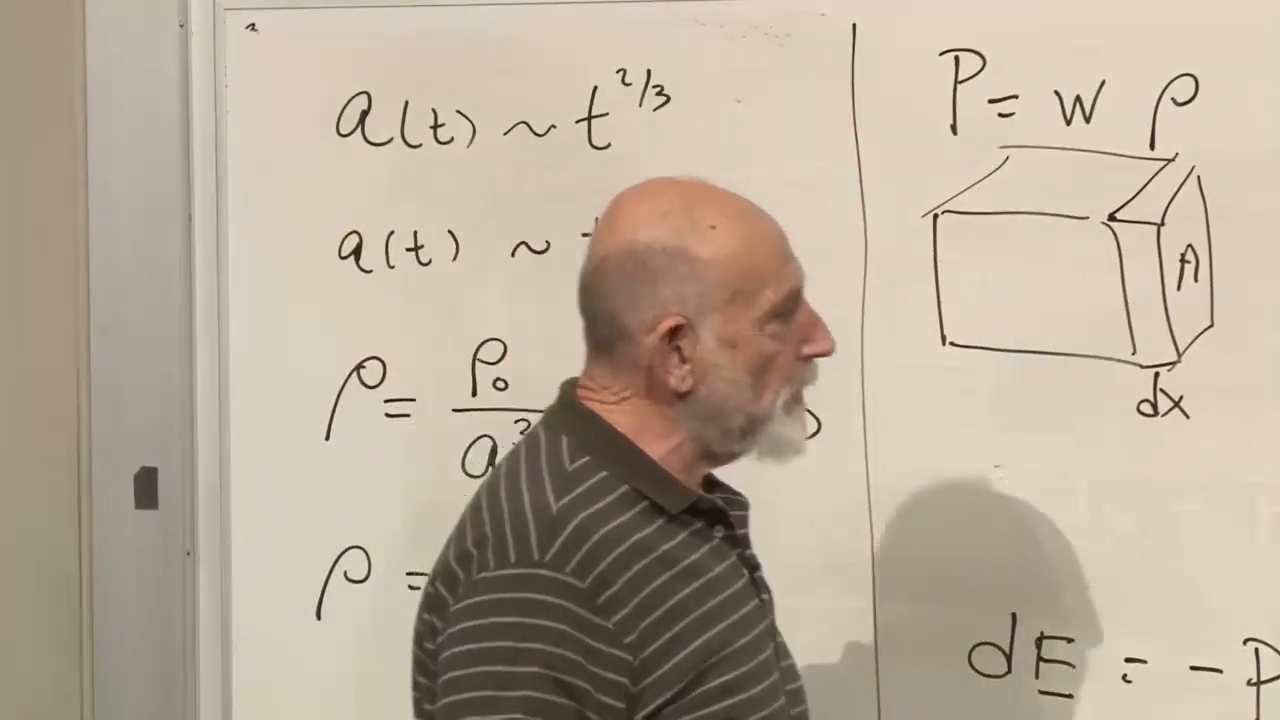
\includegraphics[width=0.86\textwidth]{lecture_05_figure_03.png}
\caption{Phương trình trạng thái, các quy luật tỉ lệ của mật độ đã được ôn lại, và chiếc hộp nhiệt động học trên cùng một bảng. Giảng viên che khuất một phần nội dung đã viết trước đó, nên hình này được dùng để thể hiện bố cục và các phương trình còn nhìn thấy được hơn là như một bản chép đầy đủ.}
\label{fig:c05-box-board}
\lectureframe{00:13:39.612}
\end{figure}

Phía trái của bảng mang các quy luật tỉ lệ vũ trụ học đã được ôn lại; phía phải bắt đầu lập luận về chiếc hộp. Đọc cùng nhau, nội dung nhìn thấy được liên kết thành
\begin{equation}
\rho_{\text{matter}}=\frac{\rho_0}{a^3},
\qquad
\rho_{\text{rad}}=\frac{\rho_0}{a^4},
\qquad
P=w\rho.
\end{equation}
Nhiệm vụ của ta là suy ra hai định luật mật độ từ phương trình trạng thái.

Một mặt có diện tích \(A\). Dời nó ra ngoài một đoạn \(dx\), khi đó
\begin{equation}
dV=A\,dx.
\end{equation}
Áp suất là lực trên một đơn vị diện tích, nên lực tác dụng lên mặt ấy là \(PA\). Chất khí thực hiện công \(PA\,dx=P\,dV\), và năng lượng còn lại bên trong giảm đi.
\begin{equation}
dE=-P\,dV.
\label{eq:c05-work-law}
\end{equation}
\begin{figure}[htbp]
\centering
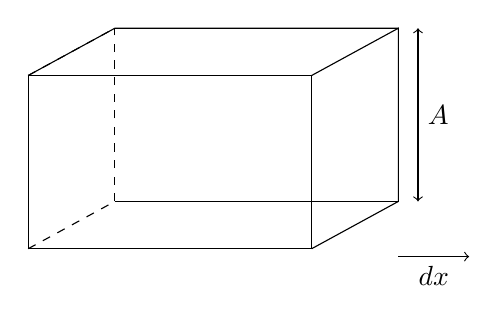
\begin{tikzpicture}[scale=1.0]
\draw (0,0) -- (3.6,0) -- (3.6,2.2) -- (0,2.2) -- cycle;
\draw (3.6,0) -- (4.7,0.6) -- (4.7,2.8) -- (3.6,2.2);
\draw (0,2.2) -- (1.1,2.8) -- (4.7,2.8);
\draw (1.1,0.6) -- (4.7,0.6);
\draw[dashed] (0,0) -- (1.1,0.6);
\draw[dashed] (0,2.2) -- (1.1,2.8);
\draw[dashed] (1.1,0.6) -- (1.1,2.8);
\draw[<->] (4.95,0.6) -- (4.95,2.8);
\node[right] at (4.95,1.7) {\(A\)};
\draw[->] (4.7,-0.1) -- (5.6,-0.1);
\node[below] at (5.15,-0.1) {\(dx\)};
\end{tikzpicture}
\caption{Bản dựng lại rõ ràng của hộp nhiệt động học, với diện tích mặt \(A\) và độ dời \(dx\).}
\label{fig:c05-box-redraw}
\end{figure}

Tổng năng lượng là
\begin{equation}
E=\rho V.
\end{equation}
Lấy vi phân, ta được
\begin{equation}
d(\rho V)=\rho\,dV+V\,d\rho.
\end{equation}
Thay vào phương trình~\eqref{eq:c05-work-law}, ta có
\begin{equation}
\rho\,dV+V\,d\rho=-P\,dV.
\end{equation}
Thế \(P=w\rho\) vào:
\begin{equation}
V\,d\rho=-(1+w)\rho\,dV.
\end{equation}
Kết quả này là bước sơ bộ dẫn đến phương trình hữu ích, nhưng vẫn chưa tới hẳn. Chia cho \(\rho V\).
\begin{equation}
\frac{d\rho}{\rho}=-(1+w)\frac{dV}{V}.
\end{equation}
\begin{figure}[htbp]
\centering
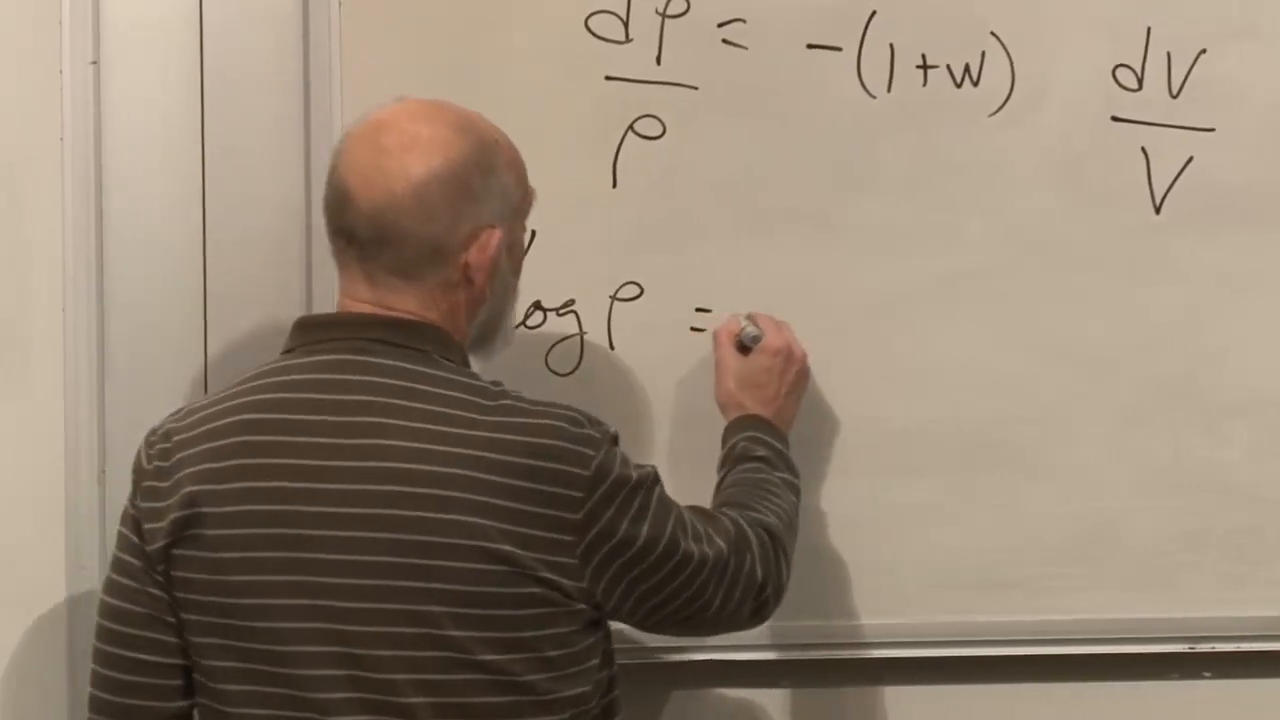
\includegraphics[width=0.78\textwidth]{lecture_05_figure_04.png}
\caption{Phương trình mật độ-thể tích đã tách và phần mở đầu của phép tích phân lôgarit. Vế phải đầy đủ được phục dựng từ đại số đi trước, chứ không phải từ các điểm ảnh bị che khuất.}
\label{fig:c05-log-board}
\lectureframe{00:15:35.600}
\end{figure}

Khung hình cho thấy phương trình đã tách và phần mở đầu \(\log\rho=\). Hoàn tất phép tích phân trực tiếp:
\begin{equation}
d(\log\rho)=-(1+w)\,d(\log V),
\end{equation}
suy ra
\begin{equation}
\log\rho=-(1+w)\log V+\text{const.}
\end{equation}
Lấy hàm mũ,
\begin{equation}
\rho\propto V^{-(1+w)}.
\end{equation}
Đây là định luật mật độ-thể tích.

Bây giờ ta quay từ chiếc hộp trở lại vũ trụ học. Chỉ di chuyển một mặt là một cách suy dẫn thuận tiện, không phải một giả thiết dị hướng. Giãn nở đồng đều theo cả ba phương cho cùng một hệ thức công, và một thể tích đồng chuyển động tỉ lệ như
\begin{equation}
V\propto a^3.
\end{equation}
Vì vậy
\begin{equation}
\boxed{\rho\propto a^{-3(1+w)}}.
\label{eq:c05-density-scaling}
\end{equation}
Trong \(d\) chiều không gian, số mũ \(3\) sẽ trở thành \(d\); phần còn lại của lập luận không đổi.

\section{Những ứng dụng đầu tiên: vật chất và bức xạ}

Giờ đây ta có thể thu lại các công thức đã ôn như những hệ quả thay vì những giả định.

Đối với vật chất phi tương đối tính, ta lấy
\begin{equation}
w=0.
\end{equation}
Khi đó
\begin{equation}
\rho\propto a^{-3},
\end{equation}
đó chính xác là định luật pha loãng của vật chất.

Đối với bức xạ, tạm thời lấy
\begin{equation}
w=\frac13.
\end{equation}
Nếu điều này đúng, thì
\begin{equation}
\rho\propto a^{-3(1+1/3)}=a^{-4}.
\end{equation}
Lũy thừa nghịch đảo phụ thêm ấy vì thế tương đương với \(w=1/3\). Bước còn chưa được giải quyết là suy ra giá trị đó từ vật lý photon.

\section{Vì sao áp suất bức xạ bằng một phần ba mật độ năng lượng của nó}

Bức xạ có thể được mô tả như sóng điện từ hoặc như các hạt không khối lượng. Hãy dùng photon và tính áp suất của một khí photon trong hộp. Hộp được vẽ trong hai chiều, nhưng chất khí và phân bố góc của nó là ba chiều. Các photon chuyển động với tốc độ ánh sáng và bật lại đàn hồi khỏi các thành giả định.

Trong chốc lát, hãy giả sử mọi photon đều có cùng năng lượng \(\epsilon\). Sự đơn giản hóa này sẽ biến mất khi cộng các đóng góp từ những năng lượng khác nhau. Gọi \(\vec{\pi}\) là vectơ động lượng của photon; ký hiệu thông dụng \(p\) được tránh vì \(P\) đã ký hiệu áp suất. Một hạt không khối lượng tuân theo các hệ thức sau.
\begin{equation}
\epsilon=c\,\pi,
\end{equation}
với \(\pi=|\vec{\pi}|\). Trong hệ đơn vị dùng trong bài giảng, \(c=1\), nên
\begin{equation}
\epsilon=\pi.
\end{equation}
Nếu \(\nu\) là mật độ số photon, thì mật độ năng lượng là
\begin{equation}
\rho=\epsilon\,\nu.
\end{equation}
Lấy trục \(x\) vuông góc với một thành. Trong một khoảng ngắn \(\Delta t\), một photon chuyển động hợp với pháp tuyến đó góc \(\theta\) chỉ chạm được vào thành nếu nó khởi đầu trong một lớp dày
\begin{equation}
\Delta x=\Delta t\cos\theta.
\end{equation}
Nếu nó phản xạ, thành phần động lượng theo \(x\) của nó đảo dấu, nên động lượng truyền cho thành là
\begin{equation}
\Delta \pi_x=2\epsilon\cos\theta.
\end{equation}
Lực là độ truyền động lượng trên một đơn vị thời gian, nên một va chạm đóng góp \(\Delta \pi_x/\Delta t\). Số photon trong lớp đó là \(\nu A\Delta x\), nhưng chỉ một nửa trong số chúng chuyển động về phía thành, nên số liên quan là \(\tfrac12 \nu A\Delta x\). Chia tổng lực cho diện tích thành \(A\), ta được
\begin{align}
P(\theta)
&=
\frac{1}{A}
\left(\frac{2\epsilon\cos\theta}{\Delta t}\right)
\left(\frac12 \nu A\Delta x\right) \\
&=
\epsilon\nu\cos\theta\frac{\Delta x}{\Delta t} \\
&=
\epsilon\nu\cos^2\theta \\
&=
\rho\cos^2\theta.
\end{align}
Kết quả này phụ thuộc vào góc vì nó chỉ là đóng góp từ các photon truyền theo một hướng.

\begin{figure}[htbp]
\centering
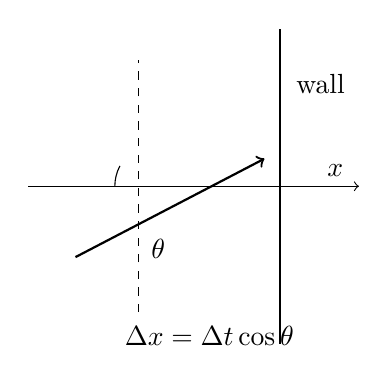
\begin{tikzpicture}[scale=1.0]
\draw[thick] (0,0) -- (0,4);
\draw[->] (-3.2,2) -- (1.0,2);
\node[above] at (0.7,2) {\(x\)};
\draw[dashed] (-1.8,0.4) -- (-1.8,3.6);
\node[below] at (-0.9,0.35) {\(\Delta x=\Delta t\cos\theta\)};
\draw[->,thick] (-2.6,1.1) -- (-0.2,2.35);
\node[below] at (-1.55,1.45) {\(\theta\)};
\draw (-2.1,2) arc[start angle=180,end angle=152,radius=0.55];
\node[right] at (0.08,3.3) {wall};
\end{tikzpicture}
\caption{Động lượng photon tới một thành dưới góc \(\theta\), hình học được dùng để suy ra áp suất bức xạ.}
\label{fig:c05-photon-pressure}
\end{figure}

Lấy trung bình trên phân bố đẳng hướng. Gọi \(\mathbf n=(n_x,n_y,n_z)\) là vectơ đơn vị dọc theo hướng chuyển động của một photon. Khi đó
\begin{equation}
n_x=\cos\theta,
\qquad
n_x^2+n_y^2+n_z^2=1.
\end{equation}
Trong một khí đẳng hướng, các giá trị trung bình của \(n_x^2\), \(n_y^2\) và \(n_z^2\) là như nhau. Lấy trung bình đẳng thức ở trên,
\begin{equation}
\langle n_x^2\rangle+\langle n_y^2\rangle+\langle n_z^2\rangle=1,
\end{equation}
và do đối xứng, mỗi hạng đều như nhau, nên
\begin{equation}
\langle n_x^2\rangle=\langle \cos^2\theta\rangle=\frac13.
\end{equation}
Vì vậy
\begin{equation}
P=\rho\langle \cos^2\theta\rangle=\frac{\rho}{3}.
\end{equation}
Do đó phương trình trạng thái của bức xạ là
\begin{equation}
P=\frac13\rho,
\qquad
w=\frac13.
\end{equation}
Thừa số \(1/3\) xuất phát từ số phương không gian cùng chia đều bình phương của vectơ đơn vị. Trong \(d\) chiều không gian đẳng hướng, cùng một lập luận sẽ cho \(\langle n_x^2\rangle=1/d\). Điều này hoàn tất phép suy dẫn vi mô đã hứa ở phần đầu.

\subsection{Những câu hỏi kiểm tra lập luận về bức xạ}

\begin{classroomqa}
\audiencequestion{Tất cả photon có cần phải có cùng năng lượng không?}
\lecturerresponse{Không. Hãy thực hiện phép tính riêng cho từng khoảng năng lượng. Mỗi khoảng đóng góp một áp suất bằng một phần ba mật độ năng lượng riêng của nó, nên khi cộng trên toàn phổ vẫn giữ được \(P=\rho/3\). Giả thiết mọi photon có cùng năng lượng chỉ nhằm giữ cho ký hiệu được ngắn gọn. \lecturetimestamp{00:39:08--00:39:36}}
\end{classroomqa}

\begin{classroomqa}
\audiencequestion{Các bức tường đen hấp thụ có cho cùng kết quả như gương hoàn hảo không, và bức tường là gì trong không gian trống?}
\lecturerresponse{Một bức tường đen ở cân bằng nhiệt sẽ hấp thụ rồi phát xạ lại bức xạ, tạo ra cùng một cân bằng động lượng trung bình. Không gian vũ trụ không có bức tường theo nghĩa đen; bề mặt ở đây là một biên tưởng tượng. Với mỗi photon đi ra ngoài, tính đẳng hướng cung cấp trung bình một thông lượng bù đi vào, nên phép tính cục bộ về dòng động lượng không thay đổi. Loại bức xạ đang được bàn trong lớp học chủ yếu là nền vi sóng vũ trụ nhiệt, mà đối với nó bức tranh cân bằng này đặc biệt tự nhiên. \lecturetimestamp{00:39:37--00:41:19}}
\end{classroomqa}

\begin{classroomqa}
\audiencequestion{Thống kê lượng tử có làm thay đổi \(P=\rho/3\) không?}
\lecturerresponse{Không. Thống kê Bose quyết định cách photon chiếm các mode cho phép và do đó quyết định phổ cùng tổng \(\rho\), nhưng ứng suất đẳng hướng của các hạt không khối lượng vẫn bằng một phần ba mật độ năng lượng đó. \lecturetimestamp{00:41:51--00:42:02}}
\end{classroomqa}

\begin{classroomqa}
\audiencequestion{Nếu các photon tán xạ lẫn nhau thì sao?}
\lecturerresponse{Tán xạ photon-photon thông thường là cực kỳ yếu, nên hiệu chỉnh của nó ở đây là không đáng kể. Ở nhiệt độ và mật độ đủ cao, các va chạm có thể tạo ra những cặp electron-positron và làm thay đổi thành phần hạt hiệu dụng cũng như phương trình trạng thái. Đó là một hiệu ứng có thật, nhưng nó thuộc về một chế độ nóng hơn nhiều so với chế độ được dùng trong lập luận này. \lecturetimestamp{00:42:02--00:43:08}}
\end{classroomqa}

\begin{classroomqa}
\audiencequestion{Diện tích tường \(A\) đã đi đâu?}
\lecturerresponse{Tích trung gian là lực do một photon tạo ra nhân với số photon đập vào tường, và số đó tỉ lệ với \(A\). Áp suất là lực chia cho diện tích, nên phép chia cuối cùng triệt tiêu \(A\). Việc gọi biểu thức trung gian là áp suất quá sớm chính là chỗ bỏ sót trên bảng; khôi phục bước từ lực sang áp suất sẽ sửa lại điều đó. \lecturetimestamp{00:43:11--00:44:01}}
\end{classroomqa}

\section{Áp suất âm và ý nghĩa của lực căng}

Cho đến lúc này, các hạt va vào các thành và đẩy chúng ra ngoài. Bức tranh đó tự nhiên dẫn đến áp suất dương, nhưng nó không bao quát hết mọi khả năng.

\begin{classroomqa}
\audiencequestion{Bản thân mật độ năng lượng có thể âm không?}
\lecturerresponse{Lý thuyết lượng tử cho phép các mật độ năng lượng âm trong những hoàn cảnh bị hạn chế, và một hằng số vũ trụ học về hình thức có thể mang một trong hai dấu. Những trường hợp như vậy đòi hỏi phải thận trọng và không phải là điểm xuất phát trực tiếp ở đây. Lối vào quen thuộc hơn là \emph{áp suất} âm, điều này có thể xảy ra ngay cả khi mật độ năng lượng là dương. \lecturetimestamp{00:44:25--00:44:59}}
\end{classroomqa}

\begin{classroomqa}
\audiencequestion{Làm sao áp suất có thể âm?}
\lecturerresponse{Trong một thế giới một chiều, một cái hộp là một đoạn thẳng. Các hạt chuyển động tự do bật lại từ hai đầu của nó và đẩy ra ngoài, tạo ra áp suất dương. Thay vào đó, hãy nối hai đầu ấy bằng một sợi dây hoặc một lò xo đang bị kéo dãn. Kéo hai đầu ra xa nhau làm lò xo kéo chúng vào trong. Lực hướng vào trong đó là lực căng, mô hình một chiều của áp suất âm. \lecturetimestamp{00:45:04--00:46:31}}
\end{classroomqa}

\begin{figure}[htbp]
\centering
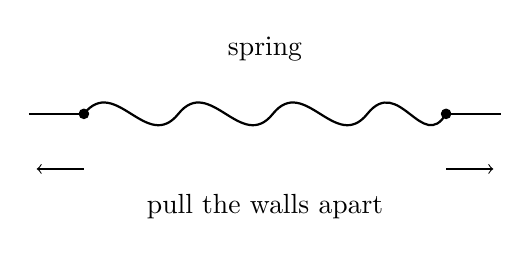
\begin{tikzpicture}[scale=1.0]
\draw[thick] (-3,0) -- (-2.3,0);
\draw[thick] (2.3,0) -- (3,0);
\draw[fill] (-2.3,0) circle (0.06);
\draw[fill] (2.3,0) circle (0.06);
\draw[thick] (-2.3,0)
.. controls (-1.9,0.5) and (-1.5,-0.5) .. (-1.1,0)
.. controls (-0.7,0.5) and (-0.3,-0.5) .. (0.1,0)
.. controls (0.5,0.5) and (0.9,-0.5) .. (1.3,0)
.. controls (1.7,0.5) and (2.0,-0.5) .. (2.3,0);
\draw[->] (-2.3,-0.7) -- (-2.9,-0.7);
\draw[->] (2.3,-0.7) -- (2.9,-0.7);
\node[below] at (0,-0.9) {pull the walls apart};
\node[above] at (0,0.55) {spring};
\end{tikzpicture}
\caption{Một lò xo một chiều như một phép loại suy cho áp suất âm.}
\label{fig:c05-tension}
\end{figure}

Theo đó, việc hạch toán công cũng đảo lại. Sự giãn nở cho phép một chất khí có áp suất dương thực hiện công và mất nội năng. Kéo ra ngoài chống lại lực căng sẽ tích trữ năng lượng trong lò xo. Tổng quát hơn, các thành phần hút nhau có thể kéo lẫn nhau và kéo biên vào trong. Vì vậy một hệ có thể có \(\rho>0\) và \(P<0\), suy ra \(w<0\), mà không hề mâu thuẫn. Khả năng này là then chốt vì năng lượng chân không có đúng mẫu dấu như vậy.

\section{Năng lượng chân không và hằng số vũ trụ học}

Năng lượng chân không được gán cho chính không gian trống. Lý thuyết trường lượng tử biện minh cho nó thông qua chuyển động điểm không của các dao động tử điều hòa gắn với các mode của trường, nhưng mô tả vĩ mô của nó không đòi hỏi ta phải giải quyết bài toán vi mô ấy. Tính chất xác định là không gian trống có cùng một mật độ năng lượng, bất kể chọn một vùng ở đâu và lớn đến mức nào.
\begin{equation}
\rho=\rho_0=\text{const.}
\label{eq:c05-vacuum-density}
\end{equation}
Nếu một vùng có thể tích \(V\) chỉ chứa năng lượng chân không, thì tổng năng lượng trong vùng đó là
\begin{equation}
E=\rho_0 V.
\end{equation}
\begin{classroomqa}
\audiencequestion{Một cái hộp có làm thay đổi mật độ chân không bằng cách hạn chế các mode trường được phép không?}
\lecturerresponse{Tổng năng lượng trong một vùng hữu hạn nhỏ hơn năng lượng của toàn bộ không gian vì vùng đó có thể tích nhỏ hơn; mật độ khối \(\rho_0\) vẫn giữ nguyên. Các biên thực có thể làm thay đổi năng lượng của các mode và sinh ra hiệu ứng Casimir, nhưng hiệu chỉnh đó chỉ quan trọng khi các khoảng cách có thể so sánh được với các bước sóng liên quan. Đó không phải là mật độ chân không quy mô lớn được dùng trong vũ trụ học. \lecturetimestamp{00:50:06--00:51:25}}
\end{classroomqa}

Đặt
\begin{equation}
\Lambda=\frac{8\pi G}{3}\rho_0.
\label{eq:c05-lambda-definition}
\end{equation}
Định nghĩa này hấp thụ tổ hợp xuất hiện trong phương trình Friedmann. Hệ thức ngược là
\begin{equation}
\rho_0=\frac{3\Lambda}{8\pi G}.
\end{equation}
Tham số \(\Lambda\) là hằng số vũ trụ học. Một thành phần dương gần như không đổi, gây ra gia tốc ở thời muộn, thường được gọi là năng lượng tối.

Sự phụ thuộc vào thừa số tỉ lệ đã được xác định rồi, nên hãy chạy ngược lập luận về cái hộp để tìm áp suất của nó. Vì \(d\rho_0=0\),
\begin{equation}
dE=d(\rho_0V)=\rho_0\,dV.
\end{equation}
Mặt khác, hệ thức công nhiệt động vẫn là
\begin{equation}
dE=-P\,dV.
\end{equation}
Nếu viết \(P=w\rho_0\), thì
\begin{equation}
dE=-w\rho_0\,dV.
\end{equation}
So sánh cho
\begin{equation}
w=-1.
\end{equation}
và do đó
\begin{equation}
P=-\rho.
\end{equation}
Phép loại suy bằng lò xo đã chuẩn bị cho dấu này. Năng lượng chân không dương có áp suất âm; năng lượng chân không âm có áp suất dương. Các phép đo thiên văn của \(w\) đặt ra câu hỏi liệu thành phần ở thời muộn có thực sự hành xử như một chân không không bị pha loãng hay không: \(w\) càng gần \(-1\) thì hành vi càng gần phương trình~\eqref{eq:c05-vacuum-density}.

\begin{classroomqa}
\audiencequestion{\(P=-\rho\) có phải là phương trình trạng thái của một vũ trụ rỗng không, và ta có thể tính \(\rho_0\) không?}
\lecturerresponse{Đó là phương trình trạng thái của không gian trống khi có năng lượng chân không hiện diện. Còn độ lớn của nó thì khó xác định hơn nhiều. Mọi trường lượng tử và mọi thang năng lượng đều có thể đóng góp, kể cả những trường chưa được phát hiện, nên không có phép tính được chấp nhận nào giải thích giá trị quan sát được. Câu đố chính không phải là làm thế nào để viết \(w=-1\), mà là vì sao tổng \(\rho_0\) lại nhỏ phi thường đến vậy. \lecturetimestamp{00:57:27--00:58:29}}
\end{classroomqa}

\section{Năng lượng chân không trong động lực học Friedmann}

Hãy tách riêng năng lượng chân không đúng như trước đây ta đã tách riêng vật chất thuần túy và bức xạ thuần túy. Với \(\rho=\rho_0\), phương trình Friedmann trở thành
\begin{equation}
\left(\frac{\dot a}{a}\right)^2=\Lambda-\frac{k}{a^2},
\label{eq:c05-vacuum-friedmann}
\end{equation}
với \(k=+1,0,-1\) tương ứng với không gian cầu, phẳng và hypebol. Dấu dương và âm của \(\Lambda\), kết hợp với ba lựa chọn của \(k\), cho ra sáu trường hợp về dấu, dù không phải trường hợp nào cũng cho phép nghiệm thực.

\begin{remark}
Bài giảng định nghĩa \(\Lambda=(8\pi G/3)\rho_0\), nên \(\Lambda\) ở đây có thứ nguyên của \(H^2\). Trong quy ước thông dụng \(G_{\mu\nu}+\Lambda_{\mathrm E}g_{\mu\nu}=8\pi G T_{\mu\nu}\), tham số tương ứng là \(\Lambda_{\mathrm E}=3\Lambda\).
\end{remark}

\subsection{Giãn nở de Sitter phẳng}

Đặt \(k=0\). Khi đó
\begin{equation}
\left(\frac{\dot a}{a}\right)^2=\Lambda.
\end{equation}
Với \(\Lambda>0\), chọn nhánh giãn nở:
\begin{equation}
\dot a=\sqrt{\Lambda}\,a,
\end{equation}
và do đó
\begin{equation}
a(t)=C\,e^{\sqrt{\Lambda}\,t}.
\end{equation}
Khi ấy tham số Hubble là hằng:
\begin{equation}
H=\frac{\dot a}{a}=\sqrt{\Lambda}.
\end{equation}
Đây là không gian de Sitter trong cách cắt lát phẳng, được đặt theo tên Willem de Sitter, người đã tìm ra nghiệm có hằng số vũ trụ học ít lâu sau khi Einstein đưa số hạng đó vào năm 1917. Nếu \(\Lambda<0\) trong khi \(k=0\), thì phương trình~\eqref{eq:c05-vacuum-friedmann} không có nghiệm thực vì \(H^2\) không thể âm.

\begin{classroomqa}
\audiencequestion{Tham số Hubble ở đây có thực sự không đổi không, và không-thời gian này có Vụ Nổ Lớn không?}
\lecturerresponse{Đối với nghiệm thuần túy trong cách cắt lát phẳng, \(H=\sqrt{\Lambda}\) là hằng đúng chính xác. Mặc dù \(a(t)\to0\) chỉ khi \(t\to-\infty\), mảnh tọa độ này không đầy đủ theo trắc địa: một số quỹ đạo hướng về quá khứ chạm tới biên của nó trong thời gian riêng hữu hạn. Vì vậy, tự bản thân công thức ấy không quyết định được câu hỏi Vụ Nổ Lớn toàn cục. Hình học de Sitter đầy đủ còn chứa nhiều hơn mảnh phẳng này, một điểm sẽ được hoãn lại cho đến khi hình học ấy được nghiên cứu chi tiết. \lecturetimestamp{01:06:54--01:08:07}}
\end{classroomqa}

Một phương trình Friedmann mang tính sơ đồ cho một vũ trụ chứa vật chất, bức xạ, độ cong và năng lượng chân không là
\begin{equation}
\left(\frac{\dot a}{a}\right)^2
=
\Lambda+\frac{C_m}{a^3}+\frac{C_r}{a^4}-\frac{k}{a^2}.
\label{eq:c05-mixed-friedmann}
\end{equation}
Ở thời sớm, khi \(a\) nhỏ, các lũy thừa nghịch đảo chi phối và năng lượng chân không là không đáng kể. Ở thời muộn, khi \(a\) lớn, hạng không đổi \(\Lambda\) chi phối. Vì vậy vũ trụ thực hiện một chuyển tiếp: lúc đầu nó có vẻ bị vật chất hoặc bức xạ chi phối, còn về sau nó tiến gần tới hành vi kiểu de Sitter.

Một hàm mũ có \(\ddot a>0\), nên sự chi phối của chân không là giãn nở gia tốc. Trong giai đoạn chuyển tiếp, gia tốc không nhất thiết phải chính xác là hàm mũ vì vật chất vẫn còn đóng góp vào phương trình~\eqref{eq:c05-mixed-friedmann}. Các quan sát vào thời kỳ của bài giảng được mô tả là bắt gặp vũ trụ trong lúc sự cạnh tranh này vẫn còn diễn ra chứ chưa ở một pha de Sitter đã thuần túy.

\section{Các câu hỏi về năng lượng chân không}

\begin{classroomqa}
\audiencequestion{Nếu năng lượng chân không là năng lượng trạng thái cơ bản, làm sao nó có thể âm?}
\lecturerresponse{Một mode dao động boson đóng góp \(+\tfrac12\hbar\omega\), còn một mode fermion đóng góp với dấu ngược lại. Năng lượng chân không ròng là một tổng trên nhiều trường và nhiều thang năng lượng, nên trước khi biết tổng thể thì cả hai dấu đều có thể xảy ra. Sự tồn tại của các đóng góp là điều tự nhiên; phần khó là giải thích phần dư cực kỳ nhỏ còn lại. \lecturetimestamp{01:12:00--01:14:12}}
\end{classroomqa}

\begin{classroomqa}
\audiencequestion{Liệu \(w=-1\) không đổi có hàm ý một big rip trong tương lai không?}
\lecturerresponse{Không. Một hằng số vũ trụ học với \(w=-1\) cho giãn nở mũ kiểu de Sitter nhưng không tạo ra sự phân kỳ tại thời gian hữu hạn gọi là big rip. Kịch bản đó thuộc về một thành phần phantom giả thuyết với \(w<-1\), trong đó mật độ tăng lên khi vũ trụ giãn nở. Ở đây không giả định có thành phần như vậy. \lecturetimestamp{01:14:13--01:15:50}}
\end{classroomqa}

\begin{classroomqa}
\audiencequestion{Liệu siêu đối xứng chính xác có làm cho năng lượng chân không triệt tiêu không?}
\lecturerresponse{Nó có thể triệt tiêu các đóng góp năng lượng không điểm vì mỗi bậc tự do boson được ghép cặp với một bậc tự do fermion. Tuy nhiên, tự nhiên không biểu lộ siêu đối xứng chính xác ở năng lượng thấp: các boson và fermion quan sát được không phải là những đối tác suy biến về khối lượng. Vì thế, sự triệt tiêu chính xác không giải thích được năng lượng chân không trong thế giới như hiện đang được quan sát. \lecturetimestamp{01:15:51--01:16:20}}
\end{classroomqa}

\begin{classroomqa}
\audiencequestion{Sự chênh lệch khổng lồ giữa một ước lượng tự nhiên của năng lượng chân không và giá trị quan sát được là gì?}
\lecturerresponse{Các hằng số phổ quát \(c\), \(\hbar\), và \(G\) xác định các đơn vị Planck. Tốc độ \(c\) giới hạn mọi tín hiệu, \(\hbar\) ấn định thang bất định lượng tử phổ quát, và \(G\) ghép mọi năng lượng với hấp dẫn. Từ chúng, người ta xây dựng được một khối lượng Planck cỡ \(10^{-5}\) gam và một chiều dài Planck cỡ \(10^{-33}\) xentimét, do đó có một mật độ năng lượng Planck xấp xỉ bằng một năng lượng Planck trên mỗi thể tích lập phương có cạnh bằng chiều dài Planck. Trong các đơn vị ấy, mật độ chân không quan sát được được nêu trong bài giảng là khoảng \(10^{-123}\), với số mũ chính xác phụ thuộc vào quy ước. Điều bí ẩn là vì sao những đóng góp vốn tự nhiên gợi ra một thang lớn hơn rất nhiều lại để lại một kết quả khác không nhỏ bé đến vậy. \lecturetimestamp{01:16:21--01:23:12}}
\end{classroomqa}

\begin{classroomqa}
\audiencequestion{Tại sao các nhà vật lý ngạc nhiên khi phát hiện một hằng số vũ trụ học khác không nếu các đóng góp chân không được kỳ vọng?}
\lecturerresponse{Những cải thiện quan sát lặp đi lặp lại đã liên tục cho kết quả phù hợp với 0. Lịch sử đó khuyến khích kỳ vọng về mặt tâm lý rằng một nguyên lý chính xác chưa biết, có lẽ trong một lý thuyết hấp dẫn lượng tử tương lai, buộc phải có sự triệt tiêu hoàn toàn. Việc phát hiện sau cùng đã đảo ngược kỳ vọng đó. Sự ngạc nhiên phản ánh nhiều thập niên các kết quả bằng không ngày càng chặt chẽ, chứ không phải một suy dẫn rằng năng lượng chân không buộc phải triệt tiêu. \lecturetimestamp{01:23:14--01:26:05}}
\end{classroomqa}

\begin{classroomqa}
\audiencequestion{Các quan sát có thể xác định liệu năng lượng tối có thay đổi theo thời gian hay không?}
\lecturerresponse{Chúng không thể loại trừ một thay đổi đột ngột trong tương lai xa, nhưng có thể so sánh lịch sử giãn nở gần đây qua hàng tỷ năm. Việc đo \(w\), hay tổng quát hơn là \(w(a)\), kiểm tra liệu mật độ có đã tiến hóa trong khoảng thời gian đó hay không. Bài giảng cho biết ràng buộc khi ấy chỉ ở mức xấp xỉ mười phần trăm; con số đó mang tính lịch sử, còn điểm cốt lõi bền vững là \(w=-1\) tương ứng với một mật độ không đổi. \lecturetimestamp{01:26:06--01:27:16}}
\end{classroomqa}

\begin{classroomqa}
\audiencequestion{Kết quả có khác đi trong một số chiều không gian khác không?}
\lecturerresponse{Cấu trúc tổng quát vẫn giữ nguyên. Trong \(d\) chiều không gian đẳng hướng, bức xạ có \(w=1/d\) và bị pha loãng như \(a^{-(d+1)}\), trong khi năng lượng chân không bất biến Lorentz vẫn có \(w=-1\). Các hệ số số học trong phương trình Friedmann thay đổi theo số chiều, nhưng sự khác biệt giữa vật chất pha loãng dần, bức xạ pha loãng dần và chân không không pha loãng vẫn còn. \lecturetimestamp{01:27:16--01:27:57}}
\end{classroomqa}

\section{Độ cong và phép tương tự cơ học}

\subsection{Độ cong dương với năng lượng chân không dương}

Lấy \(k=+1\) và \(\Lambda>0\):
\begin{equation}
\left(\frac{\dot a}{a}\right)^2=\Lambda-\frac{1}{a^2}.
\label{eq:c05-closed-vacuum}
\end{equation}
Nhân với \(a^2\),
\begin{equation}
\dot a^2-\Lambda a^2=-1.
\label{eq:c05-inverted-oscillator}
\end{equation}
Hãy xem \(a\) là tọa độ của một hạt hư cấu. Khi đó \(\dot a^2\) là hạng động năng của nó, \(-\Lambda a^2\) là một thế bậc hai lật ngược, và tổng năng lượng là \(-1\). Nhánh được phép về mặt vật lý có \(a\geq\Lambda^{-1/2}\): vũ trụ co lại từ kích thước lớn, đạt trạng thái nghỉ tại giá trị cực tiểu, rồi giãn nở trở lại.

Nghiệm chính xác là
\begin{equation}
a(t)=\Lambda^{-1/2}\cosh(\sqrt{\Lambda}\,t).
\label{eq:c05-closed-desitter}
\end{equation}
Sử dụng
\begin{equation}
\cosh(\sqrt{\Lambda}\,t)
=
\frac12\left(e^{\sqrt{\Lambda}\,t}+e^{-\sqrt{\Lambda}\,t}\right),
\end{equation}
Hàm này đối xứng theo thời gian. Tại \(t=0\), \(a=\Lambda^{-1/2}\); theo cả hai hướng thời gian nó tăng theo hàm mũ. Vì vậy, cách cắt lát đóng biểu hiện một giai đoạn co, một cực tiểu không kỳ dị, rồi giãn nở trở lại. Về mặt toàn cục, nó trông khác với cách cắt lát phẳng theo hàm mũ, nhưng cả hai hệ tọa độ đều phủ những phần của cùng một hình học de Sitter.

\subsection{Hằng số vũ trụ học âm}

Viết \(\Lambda=-|\Lambda|\). Nếu \(k=+1\), thì phương trình~\eqref{eq:c05-vacuum-friedmann} có vế phải âm với mọi \(a\), trong khi \(H^2\geq0\). Không tồn tại nghiệm FRW thực nào thuộc kiểu chân không thuần túy này.

Với \(k=-1\),
\begin{equation}
\left(\frac{\dot a}{a}\right)^2=-|\Lambda|+\frac{1}{a^2}.
\end{equation}
Nhân cả hai vế với \(a^2\),
\begin{equation}
\dot a^2+|\Lambda|a^2=1.
\label{eq:c05-negative-lambda-oscillator}
\end{equation}
Đây là phương trình năng lượng của một dao động điều hòa. Vì \(a\geq0\), một nửa chu kỳ vật lý là
\begin{equation}
a(t)=\frac{1}{\sqrt{|\Lambda|}}
\sin\!\left(\sqrt{|\Lambda|}\,t\right),
\qquad
0<t<\frac{\pi}{\sqrt{|\Lambda|}}.
\end{equation}
Vũ trụ mở bắt đầu tại \(a=0\), đạt tới \(a_{\max}=|\Lambda|^{-1/2}\), rồi quay trở lại một vụ co sụp lớn. Do đó, hình học không gian mở không bảo đảm sự giãn nở vĩnh viễn; một hằng số vũ trụ học âm có thể đảo ngược điều đó. Một giá trị dương rất lớn của \(\Lambda\) sẽ xé toạc các cấu trúc liên kết, còn giá trị âm lớn sẽ gây ra sự tái co sụp nhanh chóng.

\begin{figure}[htbp]
\centering
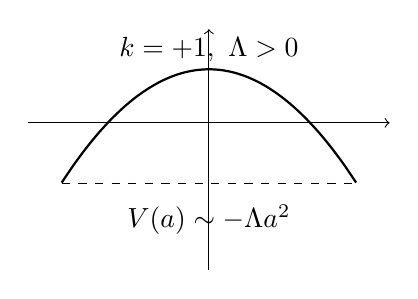
\begin{tikzpicture}[scale=0.85]
\draw[->] (-2.7,0) -- (2.7,0);
\draw[->] (0,-2.2) -- (0,1.4);
\draw[thick,domain=-2.2:2.2,smooth] plot (\x,{-0.35*(\x)^2 + 0.8});
\draw[dashed] (-2.2,-0.9) -- (2.2,-0.9);
\node at (0,-1.45) {\(V(a)\sim -\Lambda a^2\)};
\node at (0,1.1) {\(k=+1,\ \Lambda>0\)};
\end{tikzpicture}
\hspace{2em}
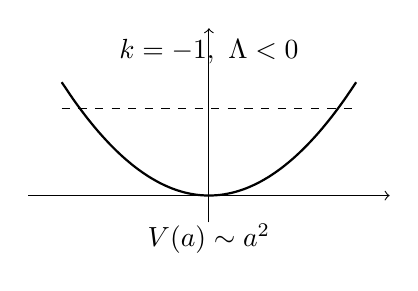
\begin{tikzpicture}[scale=0.85]
\draw[->] (-2.7,0) -- (2.7,0);
\draw[->] (0,-0.4) -- (0,2.5);
\draw[thick,domain=-2.2:2.2,smooth] plot (\x,{0.35*(\x)^2});
\draw[dashed] (-2.2,1.3) -- (2.2,1.3);
\node at (0,-0.65) {\(V(a)\sim a^2\)};
\node at (0,2.15) {\(k=-1,\ \Lambda<0\)};
\end{tikzpicture}
\caption{Các thế hiệu dụng sơ đồ cho cú nảy de Sitter đóng và sự tái co sụp của vũ trụ mở khi \(\Lambda\) âm.}
\label{fig:c05-mechanical-potentials}
\end{figure}

\begin{classroomqa}
\audiencequestion{Những phương trình Friedmann này có thật là các phương trình Einstein không?}
\lecturerresponse{Đúng. Chúng là phương trình trường Einstein sau khi tính đồng nhất và đẳng hướng rút gọn metric còn một hàm duy nhất \(a(t)\). Sự rút gọn đối xứng loại bỏ phần lớn các thành phần tensor, để lại phương trình vi phân thường này cho sự giãn nở vũ trụ. \lecturetimestamp{01:43:52--01:44:05}}
\end{classroomqa}

\begin{classroomqa}
\audiencequestion{Thừa số tỉ lệ \(a\) có thể là số phức không?}
\lecturerresponse{Không phải trong các mô hình vũ trụ học FRW cổ điển thực đang được phân tích ở đây. Thừa số tỉ lệ đo kích thước không gian và được lấy là thực, không âm. Các hình học phức hóa có thể xuất hiện trong những cách tiếp cận toán học khác, nhưng chúng không có vai trò nào trong các nghiệm của bài giảng này. \lecturetimestamp{01:44:06--01:44:21}}
\end{classroomqa}

\begin{classroomqa}
\audiencequestion{Có lý do vật lý nào khiến áp suất phải là một hàm tuyến tính của mật độ không?}
\lecturerresponse{Không. Việc lấy \(w\) không đổi là thuận tiện và tình cờ mô tả được các thành phần chính được xét ở đây. Một hỗn hợp vật chất, bức xạ và chân không không có một \(w\) không đổi qua mọi thời kỳ, và một chất nói chung có thể có \(P(\rho)\) phi tuyến. Đối với một chất lưu barotropic, \(dP/d\rho\) chi phối bình phương vận tốc âm trong các đơn vị với \(c=1\); \(w\) không đổi làm cho đạo hàm đó không đổi, nhưng tự nhiên không bị buộc phải như thế. \lecturetimestamp{01:44:21--01:45:34}}
\end{classroomqa}

\section{Những điểm cần ghi nhớ}

Phương trình trạng thái nối vật lý vi mô với lịch sử theo thời gian của thừa số tỉ lệ. Công đoạn nhiệt trong một hộp đồng chuyển động cho
\[
\rho\propto a^{-3(1+w)}.
\]
Vật chất lạnh có \(w=0\) và \(\rho\propto a^{-3}\). Dòng xung lượng photon đẳng hướng cho
\[
\left\langle\cos^2\theta\right\rangle=\frac13,
\qquad
P_{\mathrm r}=\frac{\rho_{\mathrm r}}{3},
\qquad
\rho_{\mathrm r}\propto a^{-4}.
\]

Sức căng làm cho áp suất âm trở nên dễ hiểu về mặt vật lý. Một mật độ chân không không đổi tuân theo
\[
P_\Lambda=-\rho_\Lambda,
\qquad
w_\Lambda=-1.
\]
Năng lượng chân không dương cho giãn nở de Sitter theo hàm mũ trong cách cắt lát phẳng và một cú nảy \(\cosh\) trong cách cắt lát đóng. Năng lượng chân không âm có thể khiến ngay cả một vũ trụ mở cũng tái co sụp. Trong mọi trường hợp về dấu, phương trình Friedmann có thể được đọc như một phương trình năng lượng cơ học hiệu dụng. Câu hỏi chưa được giải quyết không phải là vì sao các trường lượng tử đóng góp năng lượng chân không, mà là vì sao đóng góp ròng quan sát được của chúng gần như bằng 0 mà lại không chính xác bằng 0.
